\chapter{Manual installation}
\label{chapter:manual_install}

\section{Introduction}
The manual installation can be done on both Microsoft Windows 2000 or higher or a Linux distribution with the following software pre-installed : 
\begin{itemize}
\item Sun Java2 Standard Edition version 5.0 or higher
\item Apache Tomcat Core 5.5 or higher (other Servlet containers might work, but are not officially supported yet)
\item Postgresql 8.2.4 or higher
\end{itemize}
If you have no experience installing this software, please consult your local system administor.

\section{Manual installation steps}
\subsection{Obtaining the RegaDB software package}
The RegaDB v2.0 software package can be downloaded from our website. The regadb-package.zip (Microsoft Windows) or regadb-package.tgz (Linux) contains all necessary files to perform a manual installation of the RegaDB software.

\subsection{Configuring the Postgresql database}
Log in as posgres administrator to psql
\\
\\
Create a new role:
\\
\textbf{create user \textit{role\_name} password '\textit{role\_password}';}
\\
\\
Create a new database:
\\
\textbf{create database regadb owner \textit{role\_name};}
\\
\\
Create the schema:
\\
\textbf{create schema regadbschema authorization \textit{role\_name};}
\\
\\
Log out from psql
\\
\\
Create the Postgres database structure (this file is part of the RegaDB software package)
\\
\textbf{psql -U \textit{role\_name} regadb -f posgresSchema.sql}

\subsection{RegaDB configuration}
RegaDB requires a XML configuration file, a documented example file is available in the RegaDB software package (global-conf.xml). This config file can be placed at the default location (/etc/rega\_institute/regadb), or at an alternative location.

If you place the configuration file at an alternative location, you should define an environment variable called \textbf{REGADB\_CONF\_DIR} containing this path.
Note that this file should only be accessible by your servlet container, so please make sure only your servlet container user has read access to it.

\lstset{language=XML, caption={RegaDB XML configuration file example (with proxy settings)}}
\lstinputlisting{xml/global-conf.xml}

\subsection{Deploy RegaDB into your servlet container}
To run RegaDB v2.0 in your application server, you will need to install the regadb.war file in your application server (eg. Tomcat, JBoss, ...). This file is part of the RegaDB software package.
\\
Navigate your browser to the Tomcat welcome page (f.e. http://serverName:8080/).
\\
\vspace{0.5cm}~ \\ \centerline{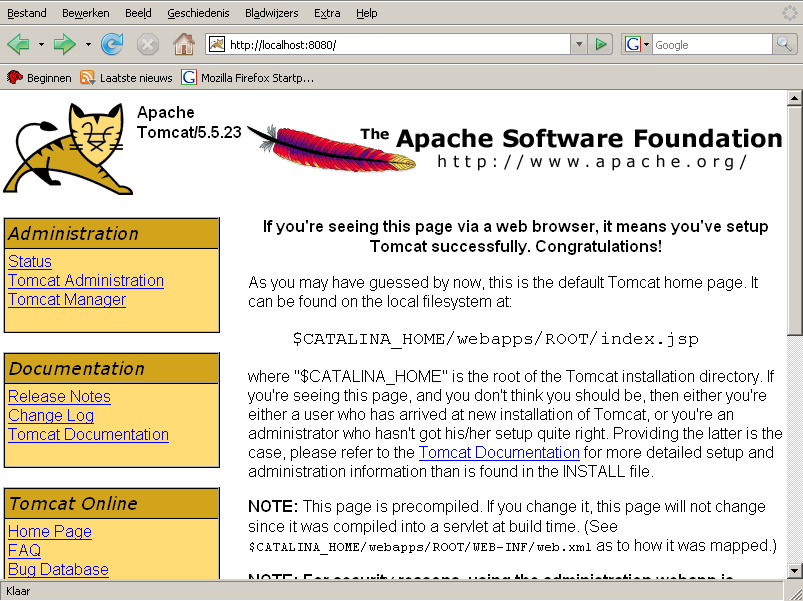
\includegraphics[width=8cm] {pics/nsis/tomcat_page.png}}
Navigate to the manager page and fill in the proper username and password.
\\
\vspace{0.5cm}~ \\ \centerline{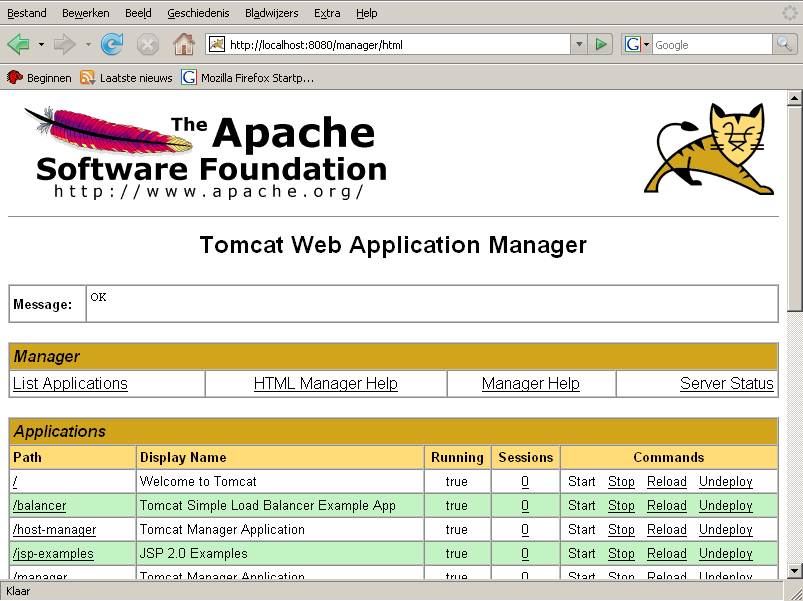
\includegraphics[width=8cm] {pics/nsis/tomcat_page_manager_1.png}}
Go to the Deploy section, browse for the regadb.war file and click \textbf{Deploy}. RegaDB will be deployed in the servlet container, this might take a few minutes.
\\
\vspace{0.5cm}~ \\ \centerline{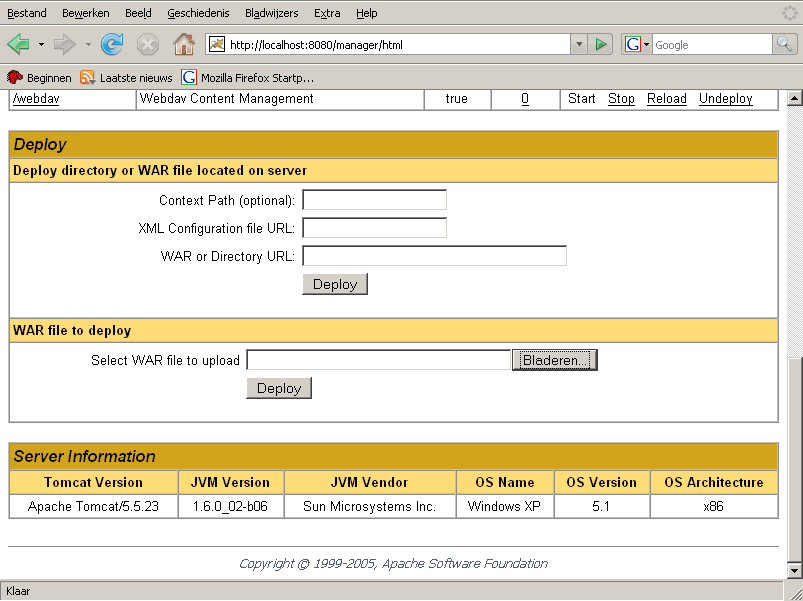
\includegraphics[width=8cm] {pics/nsis/tomcat_page_manager_2.png}}
